\documentclass[a4paper,12pt,oneside,final]{extbook}

\usepackage[utf8]{inputenc}
\usepackage[T1]{fontenc}
\usepackage{graphicx}
\usepackage{times}
\usepackage[english,swedish]{babel}
\usepackage[export]{adjustbox}
\usepackage{geometry}
\usepackage{array}
\usepackage{float}
\usepackage{caption}

\geometry{
 margin=20mm
} 

\usepackage{fancyhdr}

\usepackage{titling}
\title{Individuell rapport, TNM094}
\author{Daniel Olsson \\ Danol716\\Fleranvändar-spel med fysiska reglage}

\frenchspacing
\setlength{\parindent}{0pt}
\parskip 5pt
\usepackage{lscape}
\usepackage{color}
\definecolor{rltred}{rgb}{.5,0,0}
\definecolor{rltgreen}{rgb}{0,.5,0}
\definecolor{rltblue}{rgb}{0,0,1}

\usepackage[pdftex,
 colorlinks=true,
 urlcolor=rltblue,       % \href{...}{...} external (URL)
 filecolor=rltgreen,     % \href{...} local file
 linkcolor=rltred,       % \ref{...} and \pageref{...}
 citecolor=rltgreen,     % \cite{...}
 pdftitle={},
 pdfauthor={},
 pdfsubject={Projektrapport, TNM094},
 pdfkeywords={},
 pdfpagemode=,
 pdfstartview=FitH,
 bookmarks=true,
 bookmarksopen=false,
 bookmarksnumbered=true
        ]{hyperref}

\begin{document}

\pagestyle{empty}
\thispagestyle{empty}

\frontmatter

\maketitle

\pagestyle{fancy}

\chapter{Sammanfattning}

I en utvecklingsprocess av en produkt så möts utvecklarna av många svårigheter som kan sänka utvecklingstempot. Därför är det viktigt att innan arbetet startar ha en färdig plan över hur all arbete ska struktureras. Utseendet på planen definieras av vad för projekt som skall utvecklas. Detta är då olika projekt fungerar bättre med olika utvecklingsprocesser. Projektet som skall utvecklas är ett spel som använder sig av olika reglage för att styra spelmiljön. Dessa reglage kommer vara spakar, knappar, vridreglage, ljudsensorer och mätinstrument för väder. Innan projektet kan börjas utvecklas behövs en mängd beslut fattas och dessa involverar bland annat val om utvecklingsmetodik, mötesprinciper, spelmotor och systemarkitektur. 

Systemet har en kravlista som skall vara uppfylld och detta är vad som ligger i grunden till de flesta beslut. Då kravlista inte specificerar hur slutprodukten skall se så driver detta på att systemet skall vara öppet för förändringar. Detta ger att agil utveckling är passande för systemet. Tillsammans med agil utveckling så kommer en scrum liknande struktur användas för hur kraven skall hanteras samt hur arbetet kommer struktureras upp.
 

  



\tableofcontents

\cleardoublepage
% \phantomsection
\addcontentsline{toc}{chapter}{\listfigurename}
\listoffigures

\cleardoublepage
% \phantomsection
\addcontentsline{toc}{chapter}{\listtablename}
\listoftables

\mainmatter

\chapter{Inledning}
\label{ch:inledning}

För att utveckla ett större projekt krävs bra rutiner, principer och ledarskap. Då alla projekt inte är identiska krävs en noggrann analys för att definiera dessa.

\section{Bakgrund}
 Processen för att utveckla ett system är ofta komplex och lång. Det finns därför många olika metodiker som utvecklare kan jobba enligt för att maximera effektiviteten. En bra metodik genererar att processen blir mer överblickbar, redundant och anpassningsbar. Då varje projekt inte är likt ett annat så går det inte alltid att följa en specifik metodik och därför behövs varje aspekt i ett projekt analyseras för att se vad som passar bäst. En arbetsprocess som inte lämpar sig för ett projekt kan få ödesdigra effekter i form av overhead\footnote{Overhead - Tid som går åt till administrativa uppgifter eller andra indirekta kostnader.} och kan till och med resultera i ett nedlagt projekt.

Förutom arbetsprocessen så är systemets arkitektur och kodens struktur viktig för hur effektivt ett system är och hur lätt det är att underhålla det efter flera år. Skall ett system ha lång livslängd krävs det bra en bra struktur som gör det enkelt att sätta sig in i produkten utan att ha varit med och utvecklat den från början.
\section{Syfte}

Syftet med detta arbete är att analysera och rekommendera en passande utveckling plan för ett specifikt projekt. Detta innebär att ge förslag på utvecklingsmetodik, systemarkitektur och projekthantering. Planen är en rekommendation och kan ändras under projektets gång om planen inte fungerar eller om ett bättre plan uppstår. 

Projektets slutprodukt kommer vara ett spel med inriktning mot barn som skall användas på museum och vetenskapscentrum runt omkring i Sverige. Slutprodukten skall använda sig av flera externa reglage som används för att styra och kontroller olika aspekter av spelmiljön. Spelet kommer vara uppbyggd att det inte kommer gå att spela ensam utan det behövs minst två spelare för att lyckas klara av det. Detta är för att öka integration  och samarbete mellan barn i en fysisk miljö. Spelet kommer gå ut på att ta sig från punkt A till punkt B med hjälp av de olika reglagen som förändrar miljön och det kommer möjliggöra en passage för spelarobjektet. Det kommer även finnas reglage som styras av ljud där till exempel ett barn måste viska mot en punkt på skärmen för en vis effekt skall hända. Förutom mänskliga input kommer det hämtas data från vädret utomhus. Det menas med att om det snöar utomhus kommer det snöa inne i spelet och detta kommer ge en mer genuin känsla för spelet. För att öka återspelsvärdet kommer inga fasta nivåer användas utan de kommer att genereras automatiskt så att varje spelomgång är unik.



\section{Frågeställning}
För att kunna analysera vilken arbetsprocess som passar utvecklingsteamet bäst måste det definieras vad som är önskvärt med en arbetsprocess. Det som eftersträvas är minskad tidsåtgång, högre kvalitet och att  funktionalitet på slutprodukten fungerar som den skall. Detta kan formuleras med följande frågeställning: 
\begin{itemize}
	\item Vilken system-arkitektur passar vår slutprodukt? 
	\item Är det ekonomiskt hållbart att bygga en egen spelmotor\footnote{Spelmotor - Ett program eller bibliotek som ger utvecklaren redan klara funktioner för hantering av grafik och inmatning från användaren.} framför att betala licens för en extern?
	\item På vilka sätt går det att använda sig av refaktorering\footnote{Refaktorering - Förbättra redan skriven kod så att funktionaliteten är samma fast koden fungerar bättre eller är mer förståelig\cite{Fowler2000rit}.} i ett projekt som inte involverad gammal kod?

\end{itemize}
Denna frågeställning skall kommer besvaras för att kunna ge rekommendationer hur arbetsprocess skall ske.

\section{Avgränsningar}
Inga avgränsningar har gjort för detta arbetet.


\chapter{System och tekniska lösningar}
För att utveckla produkten måste vissa tekniska ställningstaganden göras. Detta involverar till exempel om teamet skall utveckla funktionalitet själva eller köpa in det, val av utvecklingsmiljö och hur produkten skall utvecklas.

\section{Grundläggande, initiala krav och systembegränsningar}
Slutprodukten kommer vara ett spel som där fokus kommer vara lärande men samtidigt vara kul och utmanande. Spelet skall stå på som utställning på museum och vetenskapscentrum runt omkring i Sverige och detta ställer vissa krav på systemet. I samarbete med kunden tog en kravlista fram över slutprodukten vilket kan ses i sitt fullo i bilaga \ref{Kravspecifikation}. De viktigaste punkterna som definierar slutprodukten kan ses nedan.

Slutprodukten skall:
\begin{itemize}
	\item minst använda sig av 3 externa knappar och 1 extern spak.
	\item kunna brukas av en normalbegåvad sexåring.
	\item kräva minst två spelare för att vara spelbart.
	\item ha rymd eller programmeringstema.
	\item gå att montera för en normalteknisk person på ca 2h.
\end{itemize}

Visa av kraven ställer ett undre gräns men inget övre och detta är för att ge utvecklingsteamet lite friheter för implementationen samt möjligheten för skalning av slutprodukten.


\section{Spelmotor}
För att kunna utveckla ett spel behövs en spelmotor och då ligger frågan på om det är ekonomiskt hållbart att tillverka en egen spelmotor eller det skall köpas in en från ett externt bolag. Fördelarna med att bygga en egen är att vi har kunskapen om hur den fungerar inom projektgruppen och den kan specificeras mot det spelet som skall tillverkas. Nackdelarna är att det är väldigt tidsödslande och mycket av utvecklingstiden kommer behövas läggas på att tillverka spelmotorn. 

Fördelarna med att hyra in en spelmotor är att på kort sikt kan de vara billigare och utvecklarna kan starta från dag ett med spelutvecklingen. Nackdelarna är att utvecklarna måste sätta sig in i ett främmande programvara vilket kan generera att mycket tid kommer läggas på utbildning. Det medför också en kostnad att hyra in en spelmotor och beroende på avtal med de som har utvecklat programvaran kan det ge mer eller mindre vinst.

I detta projekt skall endast ett spel utvecklas under 1 års tid med ett begränsat antal utvecklare så då faller valet på att hyra in en spelmotor. Detta är för att det hade gått åt för mycket tid till att utveckla motorn och då skulle funktionalitet i spelet minskat.

Det finns många olika spelmotorer på marknaden och de som undersöks lite noggrannare är följande:

\begin{itemize}
	\item Unreal Engine 4
	\item Unity3D
	\item CryEngine 3
	\item HeroEngine
	
\end{itemize}

Dessa spelmotorer måste uppfylla ett antal kriterier för att det skall vara möjligt att använda de som utvecklingsmiljö för detta spel alternativt att spelmotorn har öppen källkod\footnote{Öppen källkod - Öppen källkod avser programvara vars källkod är tillgänglig att läsa, modifiera och vidaredistribuera. } så utvecklarna själva kan utveckla funktionaliteten. De kriterier som är uppsatta är följande.
Det behövs sätta upp några kriteriet för att kunna välja mellan spelmotorerna och de grundläggande kriterierna är:
\begin{itemize}
	\item Går det att bygga projekt till Windows 10.
	\item Innehava stöd för 3D, åtminstone 2.5D.
	\item Möjlighet att koppla in externa kontroller.
	\item Kostnaden för mjukvaran under 1 års utveckling skall vara under 50 000kr.
	\item Finns utbildningsmaterial?
	
\end{itemize}
Spelmotorernas möjligheter till dessa kriterier ses i tabell \ref{Spelmotorer}.

\begin{table}[h]
	\centering
	\caption{All programvara som används för att utveckla systemet}
	\label{Spelmotorer}
	\begin{tabular}{ | p{6em} | m{4em} |p{1em}| p{8em} |p{5em} |p{7em} |p{4em} |} 
		\hline
		\textbf{Spelmotor}&\textbf{Windows}  &\textbf{3D}&\textbf{Externa kontroller}&\textbf{Kostnad}&\textbf{Utbildning} &\textbf{Öppen källkod}\\ 
		\hline
		Unreal Engine 4 & Ja&Ja & Ja, via plugin&0 Euro\cite{Unreal}&Ja, Gratis& Ja  \\ 
		\hline
		Unity3D &Ja &Ja&Ja, via scripts&10500 Euro\cite{Unity}&Ja, Gratis & Nej\\ 
		\hline
		CryEngine 3 &Ja& Ja &Ja, via scripts &0 Euro\cite{CryEngine}&Ja, men mer än grundutbildning kostar& Ja \\ 
		\hline
		HeroEngine &Ja&Ja &Ingen information finns&299.95 Euro\cite{HeroEngine}& Ja, Endast forum & Nej\\ 
		\hline
		
	\end{tabular}
\end{table}

Som det ses i tabell \ref{Spelmotorer} är det endast CryEngine 4 och Unreal Engine 4 som uppfyller kraven så då grundar sig valet i priset. Båda spelmotorerna är gratis att använda och det som skiljer dem åt är att Unreal Engine 4 tar 5\% av inkomsten och medan CryEngine 4 inte tar något. Då faller valet på CryEngine 4 som spelmotor i detta projekt.

\section{Externa reglage}
För att kunna hantera flera olika reglage krävs en mikrokontroller som hanterar inmatningen för att sedan skicka signaler till datorn och spelmotorn. Valet av mikrokontroller blir en Arduino R3 och det grundar sig i att den kommer med en USB utgång för koppling till dator, den har flertalet in-och utgångar, och Arduino har en väl dokumenterad manual.

\section{Målplattform}

Projektet utvecklas för Windows 10 och ingen vikt kommer ges till att bli bakåt kompatibelt. Detta är för att slutprodukten skall stå som ett utställning objekt och kommer därmed levereras med tillhörande hårdvara inklusive dator. CryEngine 4 har funktionalitet som bygger spelet mot Windows 10.  

\section{Grundläggande system-arkitektur}
Systemet som skall utvecklas kan grovt delas in i 3 objekt:
\begin{itemize}
	\item Visualisering
	\item Inmatning
	\item Spellogik
\end{itemize}
Visualiseringen är de delar som generar en bild på skärmen, inmatningen hanterar signaler från användaren och spellogiken bestämmer bland annat om inmatningen skall hanteras eller kastas och hur det visuella skall uppdateras. Flödet mellan dessa objekt sker alltid framåt som kan ses i figur \ref{fig:System}. Visualiseringen ger data till användaren som därefter ger nya kommandon till systemet via inmatningen. Från inmatningen skickas data till spellogiken som  behandlar den och därefter uppdaterar visualiseringen. Detta system liknar strukturen för modell view controller(MVC)\cite{Design} och det är den strukturen som används för detta system på den högsta nivån. 

\begin{figure}[h]
	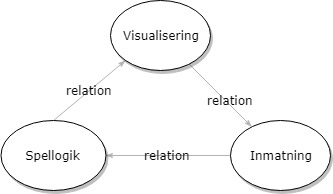
\includegraphics[width=0.5\textwidth, center]{System.jpg}
	\caption{Systemets tre objekt och deras relationer till varandra}
	\label{fig:System}
\end{figure}

Fördelar med denna struktur är att det är enklare att hitta fel i systemet och programkoden blir enklare att läsa då koden blir mer linjär och flödet är alltid riktat åt ett håll.

Visualiserings och spellogik byggs upp i CryEngine 4 och skrivs i Lua, c\# och c++ där de olika språken används till olika delar i spelmotorn så beroende på vad för funktionalitet som skall implementeras användas olika språk. Inmatningen kommer handskas av både CryEngine 4 och en Arduino R3. På Arduino R3 skrivs koden i C och kommer endast hantera de externa kontrollernas insignal för att sedan omvandla den till data som CryEngine 4 kan hantera.  

För att hantera väderdata kommer SMHI Open Data API\cite{SMHI} användas. Informationen hämtas via ett Javascript kod som ger informationen i en Json fil. Därefter hanteras Json filen i CryEngine 4 och beroende på värdet ändrat texturerna och modellerna.

\section{Standarder}
CryEngine 4 har ett begränsat antal filformat för 3D modeller som motorn klarar av att importera. Det föredragna filformatet i CryEngine är .FBX\cite{3Dmodel} vilket är det som kommer användas i detta projekt.

\section{Utvecklings-miljö}

I projektets utvecklingsfas kommer flera olika verktyg användas för att bygga och hantera slutprodukten. Dessa verktyg och dess användningsområde är samlade i tabell \ref{utvecklingsmiljö}. 


\begin{table}[H]
	\centering
	\caption{All programvara som används för att utveckla systemet}
	\label{utvecklingsmiljö}
	\begin{tabular}{ | p{9em} | m{6em} |p{23em}| } 
		\hline
		\textbf{Programtyp}&\textbf{Programnamn}  &\textbf{ Användningsområde} \\ 
		\hline
		Spelmotor &CryEngine 4 & Använd som grafikmotor och nivåskapare. \\ 
		\hline
		3D Modellering &Maya LT &Används till att skapa 3D modeller.  \\ 
		\hline
		Bildbehandlings-program &Photoshop&Används till att skapa texturer.  \\ 
		\hline
		Utvecklingsmiljö &Arduino Software &Utvecklingsmiljö för kodning mot Arduino R3.  \\ 
		\hline
		Versionshantering &Git &Används till att hålla koll på tidigare versioner och underlätta för flera programmerare att koda i samma projekt.  \\ 
		\hline
		Projekthantering &Hack n plan &Används till att hantera projektets olika delar och moment.  \\ 
		\hline

	\end{tabular}
\end{table}

Dessa programvaror skall användas av teamet, programvara till andra områden än de i tabell \ref{utvecklingsmiljö} får väljas av varje enskild utvecklare.
	



\chapter{Projekthantering}

Olika projekthanteringsmetoder ger olika fördelar och nackdelar och därför behövs projektet analyseras för att kunna hitta en metod som kan passa projektet.

\section{Utvecklingsmetodik}
Från kravspecifikationen som ses i bilaga \ref{Kravspecifikation} kan det ses att kraven inte är så hårda på vilket innehåll slutprodukten skall ha vilket genererar att utvecklingsteamet har stor möjlighet att påverka vad innehållet skall vara. Då idéer kan uppstå under projektets gång så är det bra och ha en utvecklingsmetodik som är flexibel. Därför har agil utveckling valts till detta projekt.

Agil utveckling kallas ofta för lättrörliga metoder eller iterativa metoder vilket menas att varje projekt bryts ner i mindre delar som kan utvecklas var för sig. Detta gör att det alltid finns fungerande programvara efter varje iteration. Inom agil utveckling följer man 4 st riktlinjer\cite{Sewell2012asd}:

\begin{itemize}
	\item Värderar individer och interaktion över processer och verktyg.
	\item Värderar fungerande programvara över omfattande dokumentation.
	\item Värderar kundsamarbeten över kontraktsförhandlingar.
	\item Värderar att svara på förändring över att följa en plan.
\end{itemize}
Detta kan sammanfattas med att agil utveckling är värdedrivande, det vill säga att utvecklingsteamet skall prioritera det som ger värde till slutprodukten.

Utvecklingsteamet kommer arbeta i små sprintar som är mellan 1-4 veckor långa. Under denna tiden går hela utvecklingsteamet igenom en full utvecklingscykel som involverar planering, krav analys, design, kodning, enhetstest\footnote{Enhetstest - Ett test som programmeraren själv skriver för att kolla sin kod.} och acceptanstest\footnote{Acceptanstest - Ett test där kunden granskar och ser att produkten följer kraven. }\cite{Sewell2012asd}. I slutet på varje sprint skall en hel funktionalitet vara implementerad och testad.  

En teknik som förespråkas inom agil utveckling är par programmering\cite{Sewell2012asd}. Par programmering går ut på att två programmerare sitter tillsammans och skriver kod. Den som skriver kallas föraren och den andra programmeraren kallas navigatören. Under tiden föraren skriver kod så granskar navigatören och pekar ut fel och ger råd till föraren. Detta genererar att fel kan upptäckas tidigt i processen och att koden blir mer läsbar direkt. Par programmering kommer att användas vid de viktigaste processerna så som koden för att kontrollera de externa kontrollerna samt de automatiska genererade nivåerna. 

\begin{figure}[h]
	\includegraphics[width=0.7\textwidth, center]{agil.png}
	\caption{Arbetsprocessen där fokus är på att ha färdig programvara.}
	\label{fig:refaktorering}
\end{figure}

Inom agil utveckling förespråkas att så fort som möjligt ha en fungerande programvara för att sedan refaktorera den ifall det finns ett behov. Refaktorering behövs då koden är dåligt optimerad eller om den luktar dåligt som är ett utryck som myntades av Kent Beck\cite{Fowler2000rit}. Kent Beck och Martin Fowler har definerat en mängd olika sätt som en kod kan lukta dåligt vilken bland annat involverar stora klasser, duplicering av kod och många argument i funktioner\cite{Fowler2000rit}. Detta är ett problem som kan uppstå i detta projekt då endast en grov plan kommer finnas. Därför kommer refaktorering att användas när det behövs under projektes gång och processen som teamet kommer jobba enligt ses i figur \ref{fig:refaktorering}.





\section{Organisation}


Detta projekt har tillgång till 10st utvecklare och en projektansvarig som har 12 månaders tid för att färdigställa slutprodukten enligt kravspecifikationen i bilaga \ref{Kravspecifikation}. Dessa 10st utvecklare är indelade i 2 grupper med olika arbetsuppgifter. Uppdelningen kan ses i tabell \ref{Utvecklare}.
\begin{table}[h]
	\centering
	\caption{Fördelningen mellan utvecklare i projektet och dess arbetsuppgifter}
	\label{Utvecklare}
	\begin{tabular}{ | p{10em} | m{3em} |p{23em}| } 
		\hline
		\textbf{Utvecklingsområde}&\textbf{Antal}  &\textbf{ Förklaring} \\ 
		\hline
		Spellogik &7st & Ansvarar för att all spellogik finns och att de externa kontrollerna fungerar med spelet. \\ 
		\hline
		Modellering och nivå editering &3st & Ansvarar för att skapa alla 3D modeller och texturer till spelet.  \\ 
		\hline
	
	\end{tabular}
\end{table}


I varje arbetsgrupp finns de tre roller och dessa är scrummästare, produktägare och utvecklare. Scrummästaren ansvar är att se till att alla rutiner och principer efterföljs och skall ses som en ledare över gruppen. Produktägaren skall se till att utvecklingen av produkten sker på ett sådant sätt att värdet maximeras för kunden och har även ansvar för backloggen\footnote{Backlogg - Är en lista över allt som skall ingå i den slutgiltiga produkten. Backloggen är dynamiskt och uppdateras. }. Utvecklarna skall ha  tillräcklig kompetens inom området för att kunna slutföra en sprint utan hjälp utifrån och skall vara självstyrande\cite{Scrumguiden}. 


Projektansvariga roll är att vara scrummästare och produktägare över alla utvecklingsteam för att säkerställa att alla teamen jobbar mot samma mål och att ingen del av teamen ligger efter.

\section{Tidsplan}
Detta projekt har ett tidsspann på 52 veckor för att få fram en slutprodukt enligt kravspecifikation i bilaga \ref{Kravspecifikation}. Projektet har en start i vecka 12 2018 och kommer att slutföras vecka 11 2019 då den slutgiltiga produkten skall visas upp för kunden. 

Arbetsgruppen kommer jobba i sprintar där varje sprint är mellan 1-4 veckor. Till varje sprint diskuterar produktägaren och utvecklingsteamet om vad som skall göras under nästa sprint och längden på denna. Målet efter varje sprint är att kunna visa upp ett färdigt delsystem. 

För att ge frihet till utvecklingsteamet så har en grov tidsplan tagits fram som endast visar när vis funktionalitet skall vara implementerad och vad som sker mellan deadlines är det upp till produktägaren att se till att rätt saker sker.  Tidsplanen kan ses i figur \ref{fig:tidsplan}.

\begin{figure}[H]
	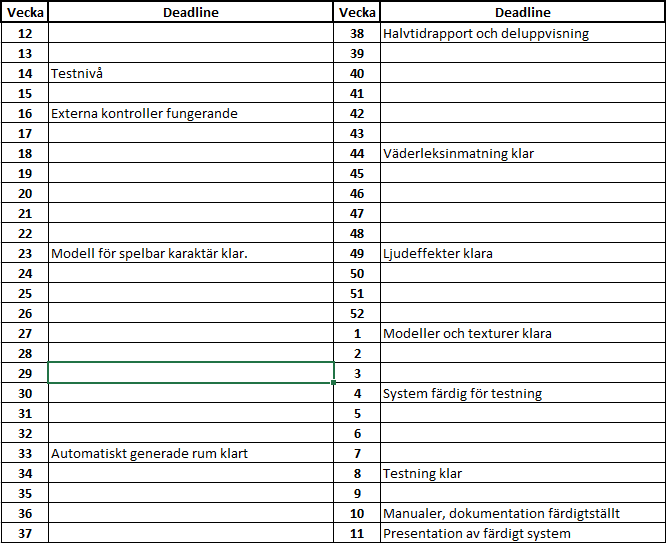
\includegraphics[width=0.7\textwidth, center]{tidsplan.jpg}
	\caption{Den grova tidsplanen för projektet.}
	\label{fig:tidsplan}
\end{figure}
Det faller mycket ansvar på produktägaren att se och bryta upp deadlines i poster så utvecklingsteamen har något att jobba mot.


\section{Milestones och leverabler}
 Från tabell \ref{fig:tidsplan} ses det flera olika deadlines. De viktigaste är testnivå, halvtidsrapport, systemfärdigt för testning, och manualer.
 
 Testnivå deadlinen innebär det finns en spelbart spel som alla utvecklare kan testa sina funktioner mot. Finns inte denna så finns det ingen möjlighet att göra integrationstest andra delar i systemet.
 
 Halvtidsrapporten skall innehålla information om vilken funktionalitet som är klar samt om denna funktionalitet skall fortsätta utvecklas när det finns slack\footnote{Slack- Inplanerad tid för missberäkningar och andra oförutsägbara händelser.}. Halvtidsrapporten skall också innehålla en prognos för det fortsätta arbetet för att se om alla krav kommer hinnas med. Detta är för att kunden och produktägaren skall kunna analysera och se om vilka poster som är viktigast att fortsätta med.
 
 Att systemet skall vara färdigt för testning betyder att systemet skall gå in i beta testning\footnote{Beta testning - När programvara blir testat av utvalda användare utanför utvecklingteamet.}. Systemet kommer inte utvecklas med ny funktionallitet utan utvecklarna kommer rätta till buggar som har hittats under testningarna. 
 
 I slutet på projektet skall alla manualer och annat dokumentation vara färdig. Detta kan involvera installationsmanual, kod dokumentation och rapport över systemet.


\chapter{Rutiner och principer}

För att öka produktiviteten och samarbetet mellan alla utvecklare sätts rutiner upp. Dessa skall hjälpa att all kod och dokument följer ett särskilt mönster så att det inte blir misskommunikation mellan utvecklare.

\section{Mötesprinciper och rutiner}

Det kommer ske tre olika sorters möten och det är veckomöte, sprintmöte och scrummöte. Där de alla olika mötena har ett speciellt upplägg.  

Veckomöte är ett möte som infaller varje måndag klockan 08:15 för att säkerställa att alla utvecklare vet vad de ska göra den kommande veckan samt att påminna om eventuella kundmöten. Detta mötet skall ta ungefär 30 min.

Under sprintmötet bestämts vad som skall ske under nästa sprint och vad som skall färdigställas. Arbetsuppgifter delas ut bland de ansvariga utvecklarna som sedan vidarebefordrar ut dte till sina arbetsgrupper. Detta mötet är beräknat till ca 180 min.

Scrummöterna sker i varje utvecklingsgrupp och där tas aktuella problem upp samt redovisar alla hur långt de har kommit med sprinten.  Detta mötet är beräknat till ungefär 5 min.

\section{Kravhantering och -sårning}
Kraven kommer hanteras i en backlogg som produktägaren i varje team ansvarar över. Alla krav i backloggen kommer att grupperas så det enkelt går att se vilka poster som tillhör vilket team samt vilka poster som påverkar alla. 

Alla poster kommer hanteras av verktyget hack n plan som har ett kanban\footnote{Kanban - Ett utryck från Japan där de satte upp en tavla med alla olika produkter och var de var i en process.} upplägg. I detta verktyg kan de ses vem som jobbar på de olika delarna i projektet samt var alla poster är i utvecklingsprocessen. Hack n plan skall uppdateras 1 gång av dagen av varje utvecklare.

Projektansvarige har ansvarat att se till att kraven fortfarande är relevanta för kunden och att se till att kunden är med i processen och ser produkten utvecklas i alla steg.

\section{Versionshantering, -system och rutiner}
Versionhantering är en viktigt pelare i ett projekt för att enklare kunna se vem som gjort vad och ha möjligheten att gå tillbaka till äldre versioner. I detta projekt kommer Git användas som versionhanteringsprogram tillsammans med en extern server. Den externa serven kommer ligga på Gitlab och det beslutet grundar sig på tidigare licenser.

Git fungerar så att man lägger till ändringar i en staging area\cite{Staging} där de kan formateras och  granskas för att sedan via en commit godkännas för att skickas till den externa servern. En bild över förloppet ses i figur \ref{fig:Gitcommit}.

\begin{figure}[H]
	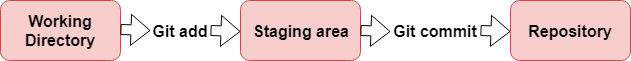
\includegraphics[width=0.8\textwidth, center]{Git.png}
	\caption{De olika stegen i git innan koden skickas till den externa servern. \cite{Staging}.}
	\label{fig:Gitcommit}
\end{figure}
Fördelen med git är att man kan jobba i en så kallad branch. En branch kan liknas med en gren som vid en vis tidpunkt är identiskt med en huvudgrenen(även kallad master) och på grenen kan ändringar ske utan att ändra på huvudgrenen. Sen när ändringar är gjorda i sitt fullo på en branch så sätt den samman med huvudgrenen. 
\begin{figure}[H]
	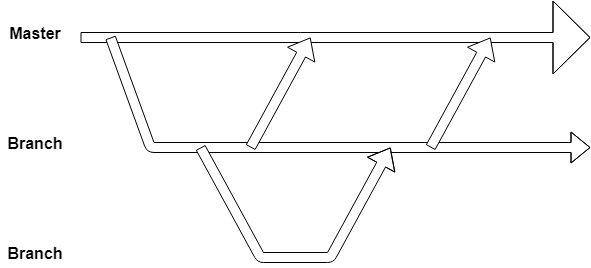
\includegraphics[width=0.8\textwidth, center]{branch.png}
	\caption{Hur en branch i git fungerar \cite{Branch}.}
	\label{fig:Gitbranch}
\end{figure}

För att undvika konflikter och trasig kod så skall några få riktlinjer följas:
\begin{itemize}
	\item Varje commit skall kommenteras kort. Nya tillägg skall kommenteras vad de gör och ändringar på gammal kod kommenteras vad som har gjorts. 
	\item Mastern skall alltid innehålla fungerande kod, alla ändringar görs på en egen branch som sedan sammanställs in i mastern när den fungerar.
	\item Alla namn på branches skall innehålla i namnet vad som utvecklas och namn på ansvarig utvecklaren. Stilen på namnet är \textit{Process\_Namn} och ett exempel kan se ut \textit{WrapperInput\_Daniel}.
	\item När en branch är fungerande skall alla test tas bort och sätts tillsammans in i mastern.
	\item Branch på en branch behöver inte ha en ansvarig utvecklare i namnet. 
\end{itemize}

Dessa punkter är riktlinjer och skulle ett specialfall dyka upp så skall detta diskuteras på ett möte.


\section{Arkitektur- och programdesign, standarder och rutiner}
All kod som skrivs skall följa uppsatta riktlinjer och för att se att all kod följer standarden kommer kod genomgångar ske. Kod genomgångarna sker genom att en utvecklare som inte har skrivit den specifika koden går in och läser och bedömer koden genom dessa riktlinjer:
  \begin{itemize}
  	\item Läsbarhet - Hur lätt koden är att läsa för en utomstående.
  	\item Struktur - Följer koden de strukturer som är uppsatta.
  	\item Välskriven - Är koden skriven på ett sätt som optimerar prestanda.
  	\item Dokumenterad - Är koden dokumenterad på rätt sätt.
  \end{itemize}
Om koden inte går igenom dessa krav får utvecklaren skriva om den för att sedan genomgå en ny kod genomgång.
\section{Dokumentationsprinciper och rutiner}
Dokumentation är en viktig del för att underlätta förståelse mellan utvecklare. Nedan beskrivs riktlinjerna för dokumentation.

\subsection{Programkod}
Programkod skall kommenteras på två olika ställen. En kommentar i toppen på varje fil och en över varje funktion. Kommentaren i toppen på varje fil skall innehålla:
\begin{itemize}
	\item Namnet på ansvarig utvecklare. Det menas med utvecklaren som är ansvarig för området och inte utvecklaren som har skrivit koden.
	\item Eventuella licenser
	\item Evuentuella tredjeparts-APIer som används.
	\item Kort sammanfattning vad filen gör.
\end{itemize}
All kommentering skall ske i Engelska.
\subsection{Möten}
Alla veckomöten skall dokumenteras i form av ett protokoll. De dagliga scrum mötena dokumenteras kortfattat i en textfil som lägg på samma server som all kod och hanteras av git. All dokumentation från möten sker på svenska.
\subsection{Slutproduktion}
Slutprodukten som är ett spel kommer dokumenteras på två sätt. En dokumentation kommer ske direkt i systemet i form av en introduktion till spelet och den andra dokumentationen är en manual hur slutprodukten skall kopplas samman. 

Indroduktionen i spelet kommer skrivas direkt i CryEngine 4 och skall fokusera på att ge en grafisk handledning istället för text. Informationen ges på de språket som användaren har valt att spela i.

Manualen kommer innehålla en stegvis beskrivning på hur alla tillbehör sätt tillsammans samt hur slutprodukten installeras. Felsökning kommer även inkluderas i manualen. Manualen skrivs på Engelska.

\section{Kvalitetssäkring}
För att säkerställa att all funktionalitet fungerar som den skall så sker det flera olika tester på olika stadier. Varje enskild programmerare kommer sköta egna enhetstest för att prova sin programkod. 

Vid de fallen där flera olika moduler samarbetar kommer ett integrationstest ske, detta kommer att göras av utvecklare som inte har utvecklad den delen som skall testas. Om det inte finns möjlighet till att använda en utvecklare som inte har utvecklat koden välj de personerna som har minst överblickande koll på koden. Detta är för att testen inte ska skrivas av vana ögon utan att testen skall prova saker som utvecklarna kanske inte har tänkt på.

Under hela processen kommer systemtest ske för att se till att all integration tillsammans fungerar.

Ingen CI-server kommer användas då uppsättningen är tidsödslande samt funktionalitet som en CI-server ger detta projekt är minimal.


\chapter{Analys och diskussion}

Vår arbetsprocess är inte perfekt och det finns risker och dessa kommer diskuteras i detta kapitel.


\section{Resultat}
Valet att hyra in en spelmotor är väldigt lättmotiverat men valet av viken spelmotor är lite mer diffus. Valet denna gång grundade sig i en ekonomiskt fråga i slutändan men det betyder inte att det kommer varit det bästa valet. Det är svårt att förutspå inlärningskurvan för utvecklarna och tar det långt tid för dem att lära sig programvaran så blir kostnaden för utbildning högre. 

När projektet går in i beta testning så är det önskvärt att kunna prova projektet på vald målgrupp men då vald målgrupp är barn så finns risk att buggar förbises. Detta är problem som lätt skulle kunna lösas av att använda sig av två olika testgrupper där barnen testar upplevelsen av systemet och den andra gruppen testar systemet efter buggar.


\section{Arbetet i ett vidare sammanhang}

Då slutprodukten skall vara riktad mot barn så är det viktigt att det finns en tanke bakom allt som finns i produkten. Barn är väldigt lättpåverkade och handlingar i ett spel kan påverka deras syn på världen. Därför är det viktigt att ha ett fokus på lärande, samarbete och förståelse. Ett exempel är att barnen får en positiv effekt att göra något som inte är tillåten så som att de måste trycka på en knapp som det står tryck ej på för att komma vidare. Detta leder till att barnen tror att det är okej att trycka på sådana knappar.


\chapter{Slutsatser}
 Systemets arkitektur bestämdes till MVC vilken är en linjär process där all information sker framåt. Detta genererar att systemet blir lättare att felsöka samt att det är enklare för utvecklarna att få en överblick hur systemets delar fungerar tillsammans.

Valet att hyra in en spelmotor visade sig väldigt självklart ur ett ekonomiskt synvinkel då flertalet av de analyserade spelmotorerna var väldigt billiga under utvecklingsdelen av projektet. Av de analyserade spelmotorerna så var de två stycken som uppfyllde alla krav som var uppsatta och valet mellan dessa grundade sig i hur stor del av avkastningen som gick till utvecklarna av spelmotorn. Valet landade då i CryEngine 4 som inte krävde någon del av avkastningen.

Refaktorering är ett bra verktyg att använda när ett system utvecklas agilt. Detta är för att det finns stora risker att koden har optimeringsproblem eller att den luktar illa och då är det bra att ha ett färdigt arbetsätt att jobba på för att optimera koden.


\bibliographystyle{vancouver}
\bibliography{referenser}

\addcontentsline{toc}{chapter}{Litteraturförteckning}

\pagestyle{empty}

\appendix


\chapter{Kravspecifikation}\label{Kravspecifikation}

	

\begin{table}[H]
	\centering
	\caption{Kravspecifikationen som projektet skall uppfylla}
	\label{Krav}
	\begin{tabular}{ | m{5em} | m{30em}| } 
		\hline
		Krav nr 1& Systemet skall minst använda sig av 3 externa knappar och 1 extern spak.   \\ 
		\hline
		Krav nr 2 & Systemet skall vara engagerande.  \\ 
		\hline
		Krav nr 3 & Systemet skall kunna brukas av en normalbegåvad sexåring. \\ 
		\hline
		Krav nr 4& Systemet skall kräva minst två spelare för att vara spelbart. \\ 
		\hline
		Krav nr 5 & Systemet skall inte ge negativ respons vid fel utan ge konstruktiv kritik till användaren. \\ 
		\hline
		Krav nr 6 & Systemet skall inte innehålla ett traditionellt poängsystem. \\ 
		\hline
		Krav nr 7& En användare skall kunna lära sig kontrollerna för systemet under 2 minuter. \\ 
		\hline
		Krav nr 8 & Systemet skall öka svårighetsgrader så att det är svårt att bemästra systemet. \\ 
		\hline
		Krav nr 9 & Systemets skall ha rymd eller programmeringstema. \\ 
		\hline
		Krav nr 10& Systemet får inte manipulera projektionsvägen. \\ 
		\hline
		Krav nr 11& Systemet skall använda grafiska hjälpmedel för att visa knappar och spakars funktionalitet.  \\ 
		\hline
		Krav nr 12& Systemet skall gå att montera för en normalteknisk person på ca 2h. \\ 
		\hline
		Krav nr 13& Systemet skall kunna användas dagligen under 2 år utan att behöva repareras \\ 
		\hline
		Krav nr 14 & Systemet skall kunna skalas om till rum i olika storlekar. Minsta storlek på rum är 2x2 meter. \\ 
		\hline
	\end{tabular}

\end{table}




\end{document}